%! Author = Administrator
%! Date = 2021/7/2

\chapter{系统测试与分析}
基于测试驱动开发的思想,在本章提出了交付的指标要求和具体测试方式,对整个系统的功能性、稳定性、并发性、可用性等多维度进行评价,确保该
系统改进的有效性,是否可以满足预期结果

\section{测试环境和工具}

\subsection{测试硬件环境}
云服务器一台
4核 / 4GB内存
容器镜像Centos7

\subsection{测试工具和方法}


\begin{figure}[H]
    \centering
    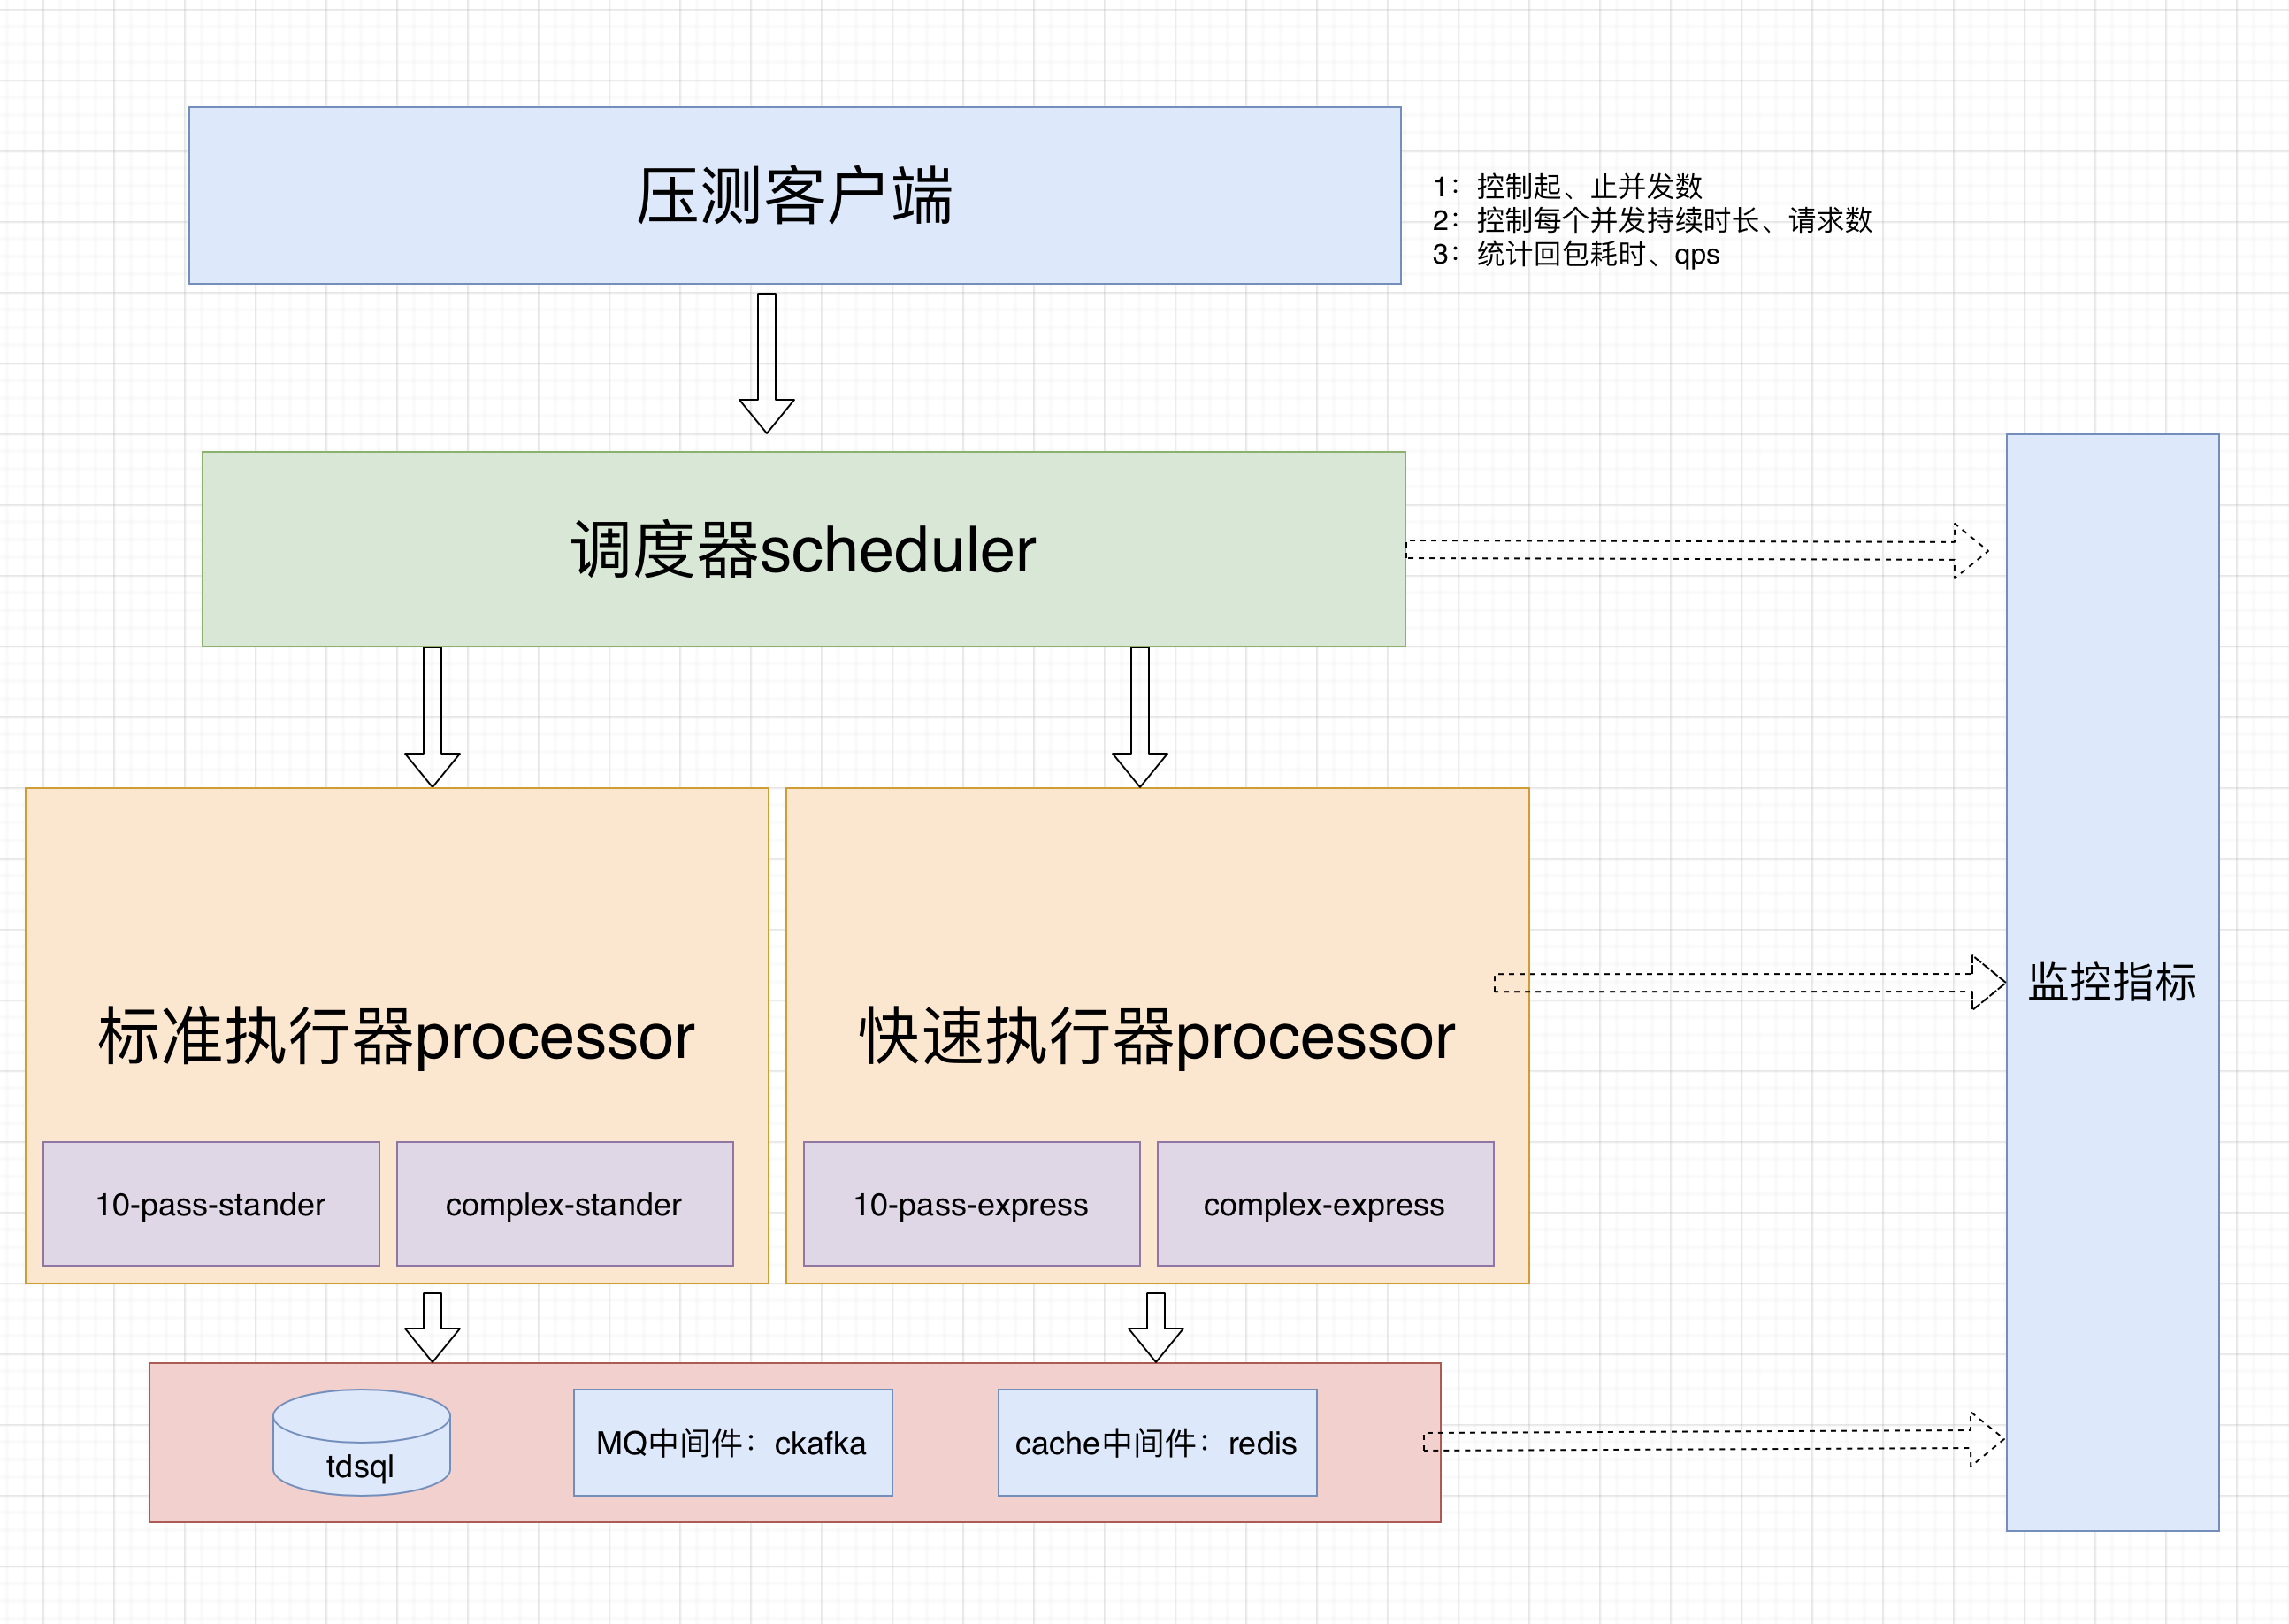
\includegraphics[width=0.9\textwidth]{press-test-2.png}
    \caption{压测计划}
    \label{fig:6-1-2}
\end{figure}

功能测试部分,通过自动化的接口测试,来保证每一次迭代上线的质量\cite{zw3}。沿用Go SDK自带的Test包,将所有发布的接口分别编写Test函数,再编写一个统一的测试
入口函数TestAll,该函数主要完成如下任务:
\begin{enumerate}
    \item 初始化构建测试数据库
    \item 读入测试用例
    \item 执行接口测试
    \item 输出测试结果
\end{enumerate}

测试数据库选用sqlite3,初始化使用migration-go, 进行数据库创建,使用go-xorm进行数据库操作(与业务DAO层保持一致)。测试用例使用JSON格式描述,
需要包含接口的输入参数,接口的预期输出。由于用例是JSON,因此断言部分主要使用jsonassert结合govaluate第三方包完成。

压力测试部分, 通过在搭建的微服务集群中创建一个容器,用于执行压力测试\cite{zw4}。


\section{功能性测试}
功能性测试部分的测试目的是为了检查设计的接口是否符合需求分析的要求。
\subsection{编排场景测试}

\begin{figure}[H]
    \centering
    \includegraphics[width=0.9\textwidth]{app0.png}
    \caption{构建DAG}
    \label{fig:6-3-2-1}
\end{figure}

如上图所示,在界面输入JSON字符串,定义了名称为n1, n2的两个工作流节点,前者对应的云资源QRN是qrn:x:1,下一个节点为n2;
后者对应的云资源QRN是qrn:x:3,为最终节点。点击“解析”,"DAGraph构造"后,可以看到生成了一个仅有2个节点有向图(dummy节点为伪节点,不参与执行)。
每一个云资源QRN都对应一个云服务的具体Serverless资源,为了简化场景,定义qrn:x:1为sum函数,qrn:x:3为send函数,该工作流的目的
是根据用户提供的输入作为sum函数的输入,计算出的结果交由send函数发送到指定容器。

\begin{figure}[H]
    \centering
    \includegraphics[width=1.0\textwidth]{app1.png}
    \caption{构建DAG结果}
    \label{fig:6-3-2-2}
\end{figure}
如上图所示,服务器的命令行输出展示了从JSON字符串解析,生成DAG的过程,在最后输出了构建好的整个DAG的节点信息,并将工作流命名为qrn:2。


\begin{figure}[H]
    \centering
    \includegraphics[width=0.7\textwidth]{app3.png}
    \caption{执行DAG}
    \label{fig:6-3-2-3}
\end{figure}
如上图所示,在输入框中以JSON字符串的形式填写测试数据k1,k2,k3为12.5,4.7,3.2。在点击执行后,执行结果显示的CostTime字段表示执行花费的时间,
Result字段表示工作流运行的结果。可以看到,结果20.4就是计算了节点1调用的函数资源sum(k1, k2, k3),并且交由节点2传递到标准输出的结果,符合预期。

\begin{figure}[H]
    \centering
    \includegraphics[width=1.0\textwidth]{app2.png}
    \caption{执行DAG结果}
    \label{fig:6-3-2-4}
\end{figure}
如上图所示,显示了服务器在执行工作流时的流程,先通过工作流qrn:2找到对应工作流,再将用户输入作为工作流Start节点的输入,再交由执行引擎逐节点执行,
每一个节点的执行都会有相应的中间输出和消耗时间,得到输出为lastNode-Result字段,值为20.4,符合预期。

以上,本小节将一个简单的场景:调用云函数并将存储结果到指定容器。定义生成了一个简单但完善的工作流,并展示了如何执行该工作流,
以及执行结果是否符合结果预期。

\subsection{接口测试}
接口测试的手段主要是通过自动化测试,提前编写测试用例,定义输入和输出。

本系统采用JSON文件定义测试用例,每一个x.request.json和x.response.json作为一组,定义序号为写的测试用例的输入和输出。
定义\@开头代表断言能力起始符,主要断言语句有\@exists():是否存在该字段,\@isEmpty():该字段是否为空字符串,
\@notEmpty():该字段是否为非空字符串,\@notExists:该字段应为不存在,\@len():该字段的长度必须满足后续给定的不等式。

涉及的接口以及其测试用例如下:

创建模板:
POST /v1/template/CreateTemplate


1.request.json:

\{

"TemplateName": "test",

"Description": "test",

"TemplateType": "EXPRESS",

%"Definition": "{\n\t\"Comment\": \"使用Pass节点演示hello world示例\",\n\t\"StartAt\": \"Hello\",\n\t\"States\": {\n\t\t\"Hello\": {\n\t\t\t\"Type\": \"Pass\",\n\t\t\t\"Comment\": \"传递\",\n\t\t\t\"Next\": \"World\"\n\t\t},\n\t\t\"World\": {\n\t\t\t\"Type\": \"Pass\",\n\t\t\t\"Comment\": \"传递\",\n\t\t\t\"End\": true\n\t\t}\n\t}\n}",

"TemplateStatus": "",

"UiConfig": ""

\}

1.response.json:

\{

"TemplateId": "\@exists()"

\}


用例解释:该用例为CreateTemplate借口的第一个测试用例,接口返回应包含TemplateId字段,否则断言不成立。后续用例皆同理。

修改模板:
POST /v1/template/ModifyTemplate

1.request.json:

\{

"TemplateId"          : "tpl-b8og5x47",

"TemplateName"        : "测试改名",

"Description"         : "测试修改描述",

%"Definition"          : "{\"Comment\":\"测试修改工作流\",\"StartAt\":\"Hello\",\"States\":{\"Hello\":{\"Type\":\"Pass\",\"Comment\":\"传递\",\"Next\":\"World\"},\"World\":{\"Type\":\"Pass\",\"Comment\":\"传递\",\"End\":true}}}",

"TemplateStatus"      : "PUBLISHED",

"UiConfig"            : ""

\}

1.response.json:

\{

    "Msg": "\@exists()"

    "ModifyTime": "\@exists()"

\}

删除模板:
POST /v1/template/DeleteTemplate

1.request.json:

\{

    "TemplateId": "\@exists()"

\}

1.response.json:

\{

    "Msg": "\@exists()"

    "DeleteTime": "\@exists()"

\}

创建工作流:
POST /v1/template/CreateFlowService

1.request.json:

\{

"FlowServiceName"        : "testFlow1443",

"FlowServiceChineseName" : "测试工作流",

%"Definition"             : "{\"Comment\":\"使用Pass节点演示hello world示例\",\"StartAt\":\"Hello\",\"States\":{\"Hello\":{\"Type\":\"Pass\",\"Comment\":\"传递\",\"Next\":\"World\"},\"World\":{\"Type\":\"Pass\",\"Comment\":\"传递\",\"End\":true}}}",

"IsNewRole"              : false,

"Type"                   : "EXPRESS",

"RoleResource"           : "qrn:qcs:asw:ap-guangzhou:45006:json:flow:test:xqb4f",

"Description"            : "description string",

"EnableCLS"              : false,

"Input"                  : ""

\}

1.response.json:

\{

"FlowServiceResource"   : "\@exists()",

"CreateDate"            : "\@exists()"

\}


修改工作流:
POST /v1/template/ModifyFlowService

1.request.json:\{

    "FlowServiceResource"   : "qrn:qcs:asw:ap-guangzhou:72248:json:flow:c139d",

%"Definition"            : "{\"Comment\":\"使用Pass节点演示hello world示例\",\"StartAt\":\"Hello\",\"States\":{\"Hello\":{\"Type\":\"Pass\",\"Comment\":\"传递\",\"Next\":\"World\"},\"World\":{\"Type\":\"Pass\",\"Comment\":\"传递\",\"End\":true}}}",

    "FlowServiceName"       :  "zzz",

    "FlowServiceChineseName":  "测试改中文名",

    "IsNewRole"             :  false,

    "Type"                  :  "STANDARD",

    "RoleResource"          :  "qcs::cam::uin/100011023428:roleName/zzz\_1304034199\_c139dk16",

    "Description"           :  "测试修改描述",

    "EnableCLS"             :  false

\}

1.response.json:

\{

"FlowServiceResource": "\@notEmpty()",

"UpdateDate": "\@notEmpty()"

\}

删除工作流:
POST /v1/template/DeleteFlowService

1.request.json:

\{

    "TemplateId": "\@exists()"

\}


1.response.json:

\{

    "Msg": "\@exists()"

    "DeleteTime": "\@exists()"

\}


开始执行:
POST /v1/scheduler/StartExecution

Parallel模式、Normal模式

1.request.json:

\{

"Input": "\@exists()"

"Name": "\@notEmpty()"

\}


1.response.json:

\{

"ExecutionQrn": "\@notEmpty()"

\}


获取任务状态:
GET /v1/processor/GetTaskStatus

1.request.json:

\{

"TaskIds": "\@exists()"

\}


1.response.json:

\{

"TaskStatus": "\@exists()"

"Error": "\@notExists()"

\}

提交任务:
POST /v1/processor/SubmitCmd

1.request.json:

\{

\}

1.response.json:

\{

\}

获取模板列表
GET /v1/template/DescribeTemplates

1.request.json:

\{

"TemplateIds": [
"tpl-b8og5x47",
"tpl-bcquf84m"
],

"Offset": 0,

"Limit": 10,

"Filters": [\{

    "Name": "TemplateType",

    "Values": ["QUICK\_START"]
\}]

\}


1.response.json:

\{

\}

获取工作流列表:
GET /v1/template/DescribeFlowServices

1.request.json:

\{

"Offset": 0,

"Limit": 10,

"Filters": [\{

"Name": "Type",

"Value": "EXPRESS"

\}]

\}

1.response.json:

\{

"TotalCount": "\@exists()",

"FlowServiceSet": "\@exists()"

\}

获取工作流详情:
GET /v1/template/DescribeFlowServiceDetail


1.request.json:

\{

"FlowServiceResource": "qrn:qcs:asw:ap-guangzhou:12597:json:flow:c139d"

\}

1.response.json:

\{

"FlowServiceName"        :  "\@notEmpty()",

"Status"                 :  "\@notEmpty()",

"Definition"             :  "\@notEmpty()",

"RoleResource"           :  "\@notEmpty()",

"Type"                   :  "\@notEmpty()",

"CreateDate"             :  "\@notEmpty()",

"Description"            :  "\@notEmpty()",

"FlowServiceChineseName" :  "\@exists()"

\}

获取模板资源:
GET /v1/template/DescribeTemplateResources

1.request.json:

\{

"TemplateId": "tpl-c59aj3jz"

\}

1.response.json:

\{

"Resources": "\@exists()"

\}

获取部署结果:
GET /v1/template/DescribeDeployResults

1.request.json:

\{

"TemplateId": "tpl-c59aj3jz",

"ExecutionQRN": "qrn:qcs:asw:ap-guangzhou:1300746878:execution:bu5op4dq:"

\}

1.response.json:

\{

"DeployResults": "\@exists()",

"MachineQrn": "\@len()\>30"

\}

获取应用模板列表
GET /v1/template/DescribeApplicationTemplates

1.request.json:

\{

\}

1.response.json:

\{

"Templates": "\@exists()"

\}

创建用户授权信息
POST /v1/auth/CreateUserStatus

1.request.json:

\{

"uid": "123456"

\}

1.response.json:

\{

\}

获取用户状态
GET /v1/auth/DescribeUserStatus

1.request.json:

\{

\}

1.response.json:

\{

"IsNewUser": "\@exists()"

"GrantUrl": "\@exists()"

"LogFlagBit": "\@exists()"

\}

POST /v1/auth/DescribeToken

1.request.json:

\{

"RoleQRN": "\@notEmpty()"

"Region": "\@notEmpty()"

\}

1.response.json:

\{

"SecretId: "\@notEmpty()"

"SecretKey: "\@notEmpty()"

"Token: "\@exists()"

"ExpiredTime: "\@exists()"

\}


接口测试结果:

\begin{table}[H]
    \centering
    \caption{接口测试结果表}
    \label{tab:t_test_result_1}
    \begin{tabular}{lllllll}
        \toprule
        所属模块&   接口名称	& 接口描述  &测试结果 \\
        \midrule
        模板服务&   CreateTemplate	& 创建模板   &   通过\\
        &   ModifyTemplate	& 修改模板   &   通过\\
        &   DeleteTemplate	& 删除模板   &   通过\\
        &   CreateFlowService	& 创建工作流   &   通过\\
        &   ModifyFlowService	& 修改工作流   &   通过\\
        &   DeleteFlowService	& 删除工作流   &   通过\\
        &   DescribeTemplates	& 获取模板列表   &   通过\\
        &   DescribeFlowServices	& 获取工作流列表   &   通过\\
        &   DescribeFlowServiceDetail	& 获取工作流详情   &   通过\\
        &   DescribeTemplateResources	& 获取模板资源   &   通过\\
        &   DescribeDeployResults	& 获取部署结果   &   通过\\
        &   DescribeApplicationTemplates	& 获取应用模板   &   通过\\
        调度器服务&   StartExecution	& 开始执行   &   通过\\
        &   StopExecution	& 停止执行   &   通过\\
        执行器服务&   GetTaskStatus	& 获取任务执行状态   &   通过\\
        &   SubmitCmd	& 提交任务   &   通过\\
        鉴权服务&   CreateUserStatus	& 创建用户   &   通过\\
        &   DescribeUserStatus	& 查询用户状态   &   通过\\
        \bottomrule
    \end{tabular}
\end{table}



\section{非功能性测试}


非功能性测试的测试目的是验证需求分析中设计的关键功能是否正确工作。

\subsection{预测执行}


\begin{figure}[H]
    \centering
    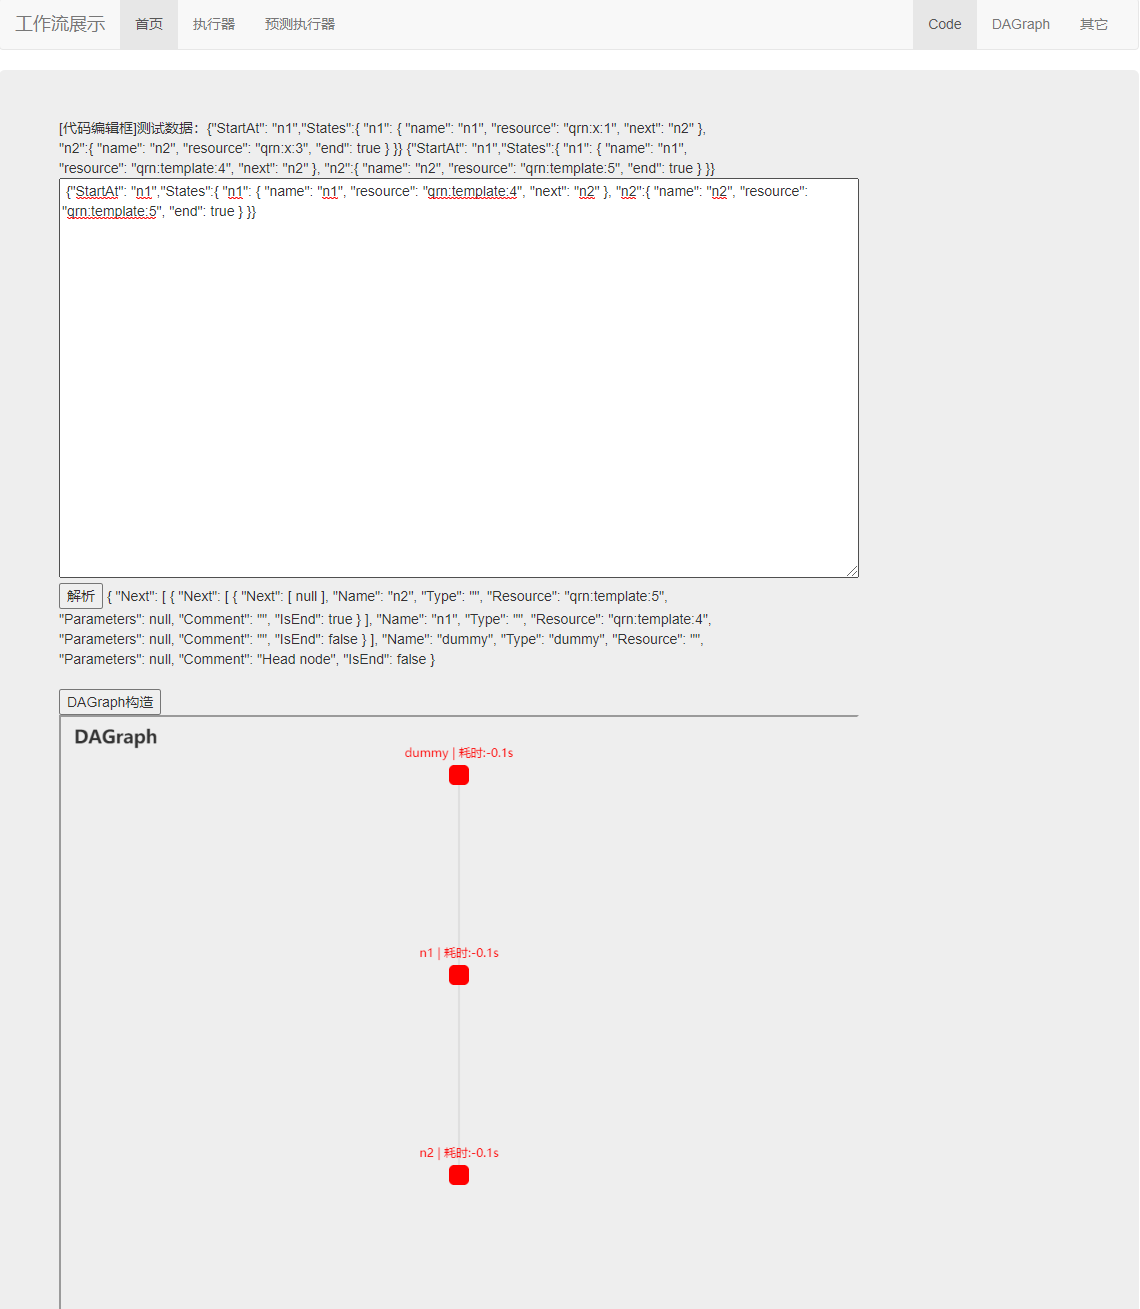
\includegraphics[width=1.0\textwidth]{p1.png}
    \caption{构建DAG}
    \label{fig:6-3-2}
\end{figure}
如上图所示,创建的测试工作流具有两个节点,分别调用qrn:template:4的资源和qrn:template:5的资源。

POST /v1/predict/ProcessPredict

\begin{figure}[H]
    \centering
    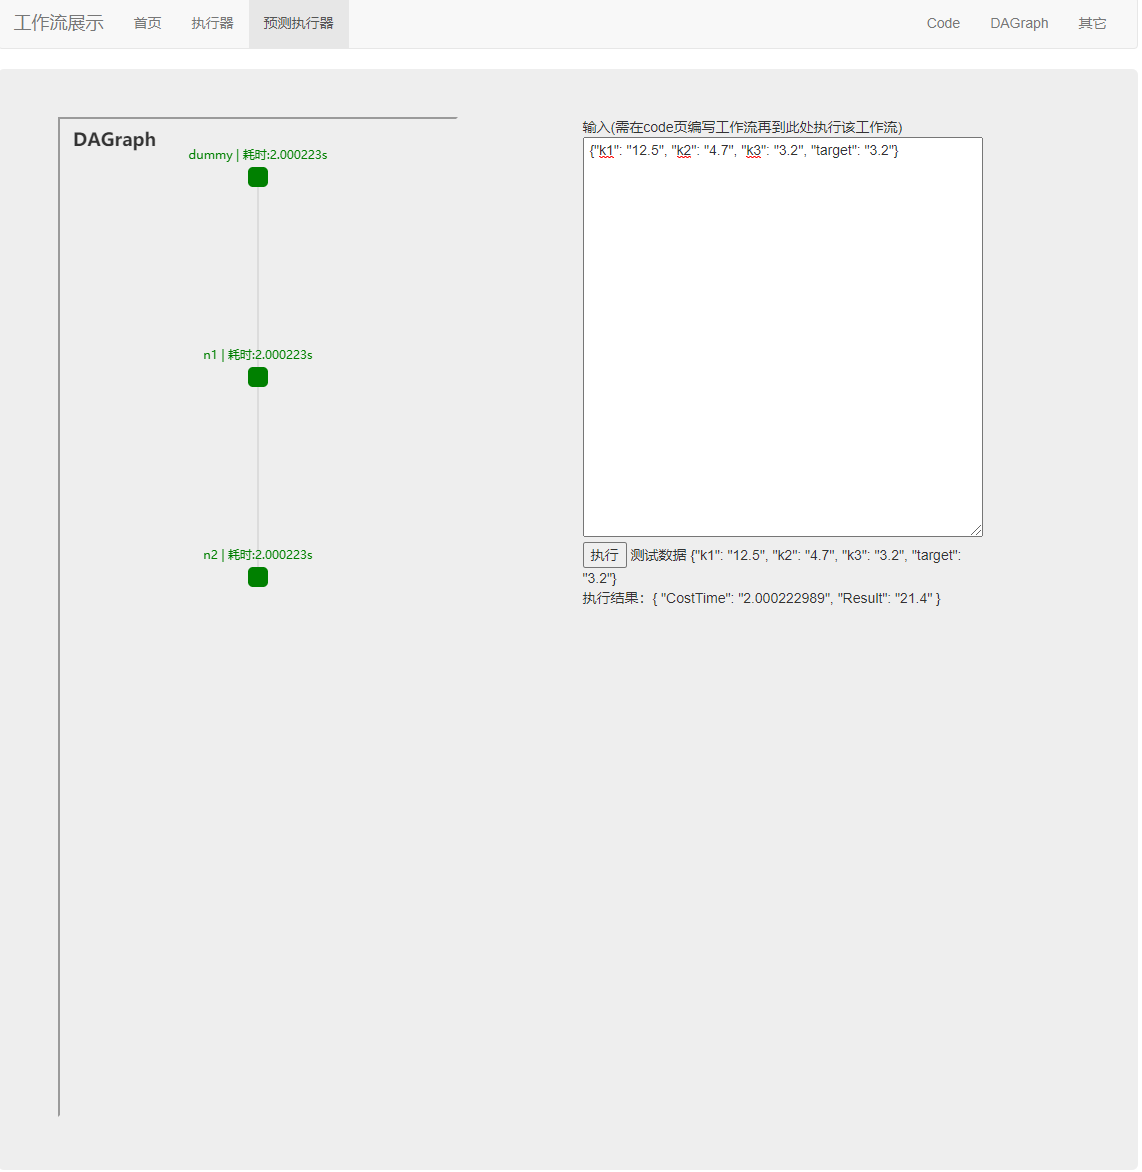
\includegraphics[width=1.0\textwidth]{p2.png}
    \caption{预测执行器执行结果}
    \label{fig:6-3-3}
\end{figure}

如上图所示,预测执行任务模式,节点1,节点2合并执行,因为是并行执行,所以时间消耗只取决于节点中最消耗时间的节点,在该例子中
是节点2,消耗2s,共计消耗2s。

POST /v1/flow/Process

\begin{figure}[H]
    \centering
    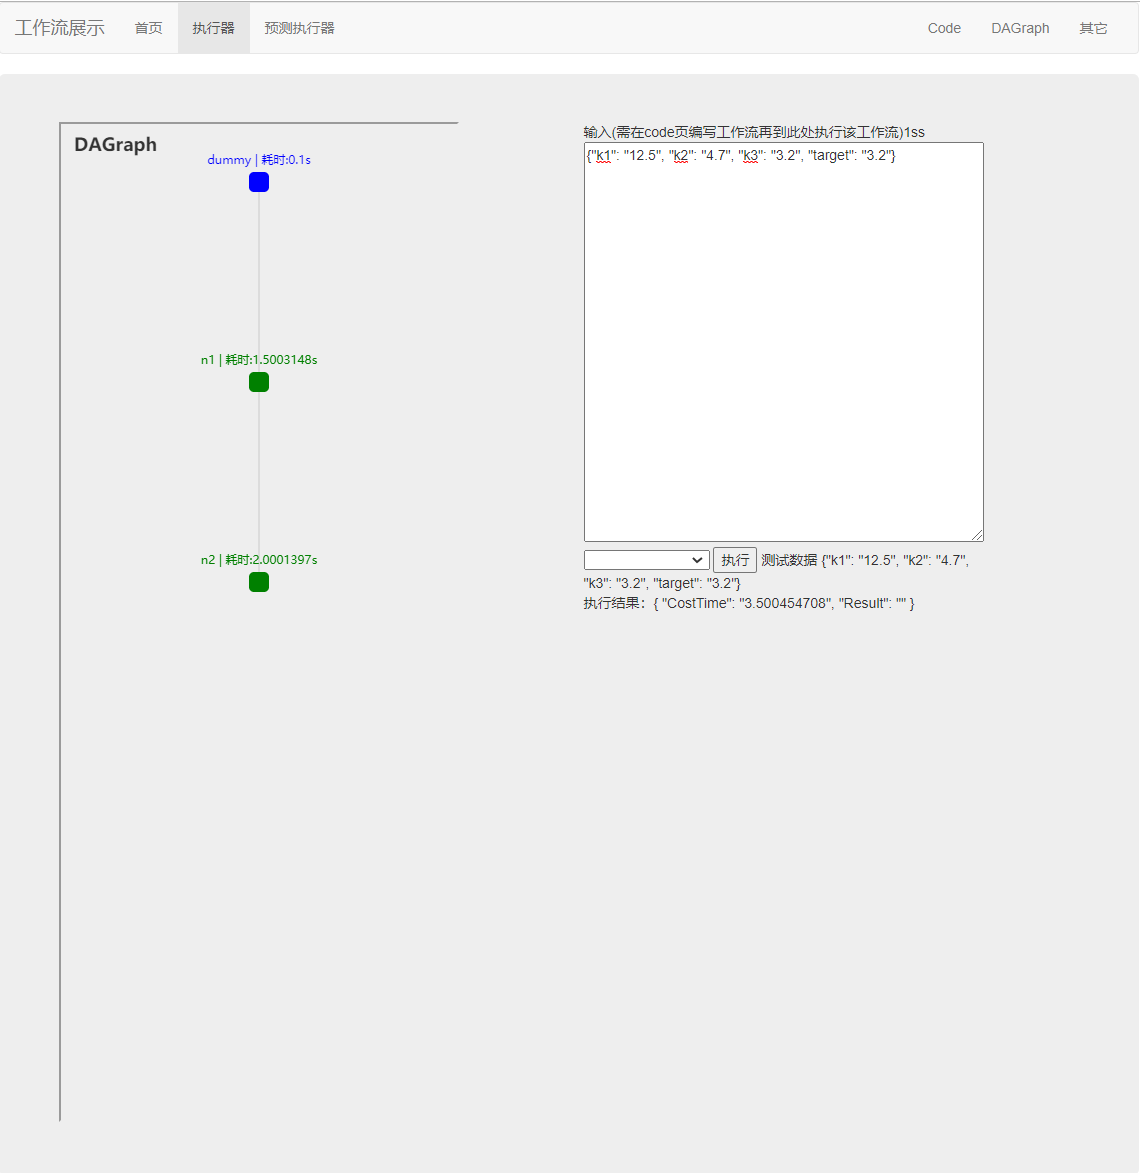
\includegraphics[width=1.0\textwidth]{p3.png}
    \caption{执行器执行结果}
    \label{fig:6-3-3-res}
\end{figure}

如上图所示,顺序执行任务模式,节点1消耗1.5s, 任务节点2消耗2s,共计3.5s。
由此可见,预测执行模式节省了1.5s的时间,只消耗了所有节点中最耗时的节点执行时长,即max(Task(i))=max(1.5s, 2s)=2s,
而顺序执行模式则是sum(Task(i))=1.5s+2s=3s。提升效率符合预期。

%POST /v1/predict/ExecutionRecord


%\subsection{动态负载探活}
%POST /v1/processor/Healthy

%\subsection{内存管理优化}
%压测,火焰图

%\subsubsection{服务降级、熔断策略}

%\subsection{自动化测试能力建设}
%go test TestAll.go


\subsection{日志巡检}

参数:threshold,超过该值的日志不进行重复输出。不填默认为10

python3 search\_error.py 10

\begin{figure}[H]
    \centering
    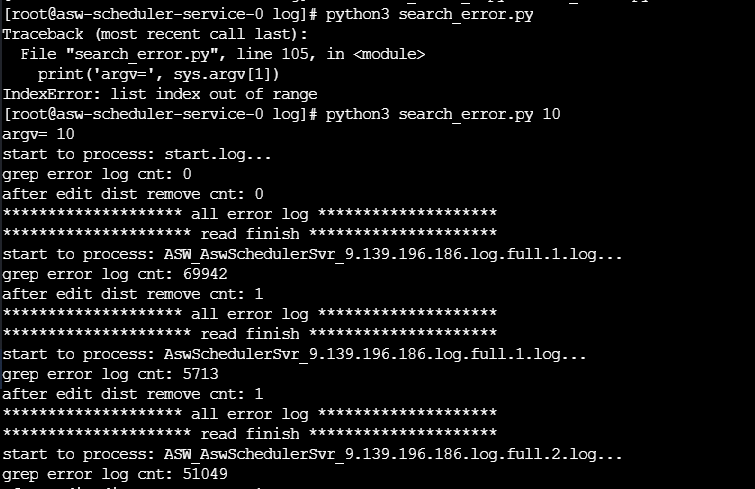
\includegraphics[width=0.8\textwidth]{log-1.png}
    \caption{巡检1}
    \label{fig:6-4-1}
\end{figure}
如上图6.5所示,程序抓取了当前目录下的所有log文件,显示了通过编辑距离算法过滤前后的日志条目数。

\begin{figure}[H]
    \centering
    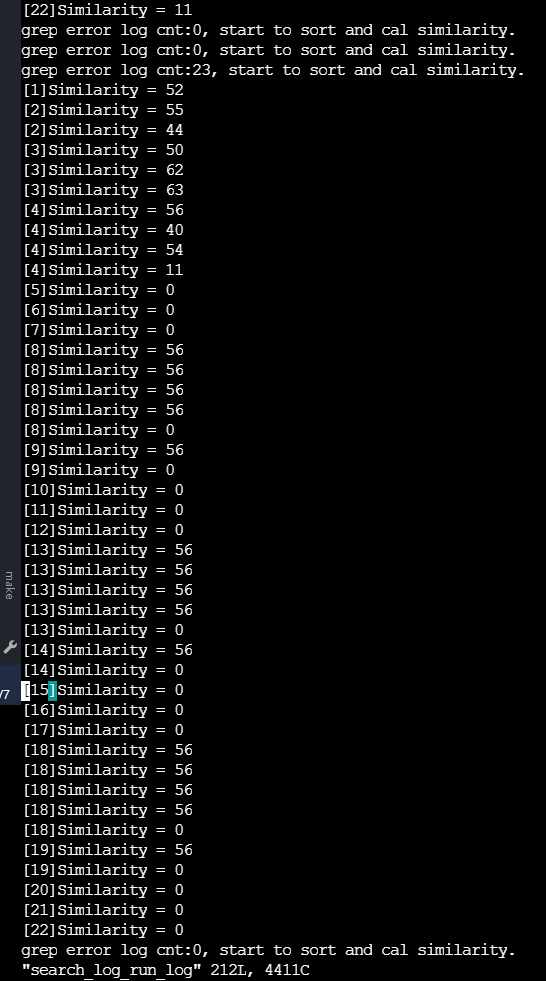
\includegraphics[width=0.7\textwidth]{log-2.png}
    \caption{巡检2}
    \label{fig:6-4-2}
\end{figure}
如上图6.6所示,程序根据每个文件读取到的日志条目,逐一进行相似度的计算,输出相似度计算的结果。

\begin{figure}[H]
    \centering
    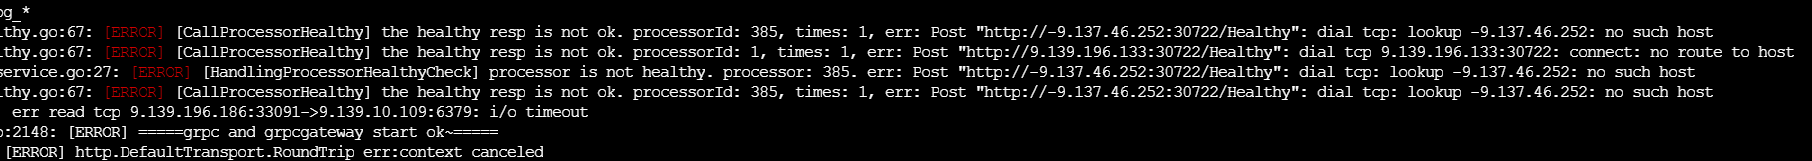
\includegraphics[width=0.9\textwidth]{log-3.png}
    \caption{巡检3}
    \label{fig:6-4-3}
\end{figure}
如上图6.7所示,程序执行完毕后查看输出文件err\_log\_*,发现共有7条数据,这是将所有日志文件中相似的错误日志过滤之后的结果。这一能力结果符合预期。

%\subsection{缓存淘汰策略}
%ZRANGE ES\_\{Machine\_Qrn\} -inf +inf
%
%经过清理算法后,每个用户工作流只存储1000条历史执行数据。


\section{压力测试}
压力测试的测试目的是检验在接受大量请求时,该系统的并发性能表现情况。

\begin{itemize}
    \item 使用https://github.com/link1st/go-stress-testing开源项目作为压力测试工具。该项目是一个go 实现的压测工具,每个用户用一个协程的方
式模拟,最大限度的利用 CPU 资源。go-stress-testing-amd -c 1 -n 100 -u localhost:8000
    \item 新建shell脚本,用于执行命令 ./go-stress-testing-amd -c $cur_con -n $req\_num -p \$curl\_file
    \item 在容器控制台执行sh press\_test.sh 100 100000 curl/stress-test-1.sh\cite{zw5}
    \item 参数\$1, \$2, \$3含义是设置并发协程数为100,请求量为100000,执行curl/stress-test-1.sh脚本里的curl请求语句(需提前写好TODO)。
    \item 对SubmitCmd接口进行业务流程的压力测试。以期调用全链路涉及的服务,目的是获取整个流程的性能开销情况。
\end{itemize}

对SubmitCmd接口压测,并发数:120 请求数:20000000
POST /v1/processor/SubmitCmd

\begin{figure}[H]
    \centering
    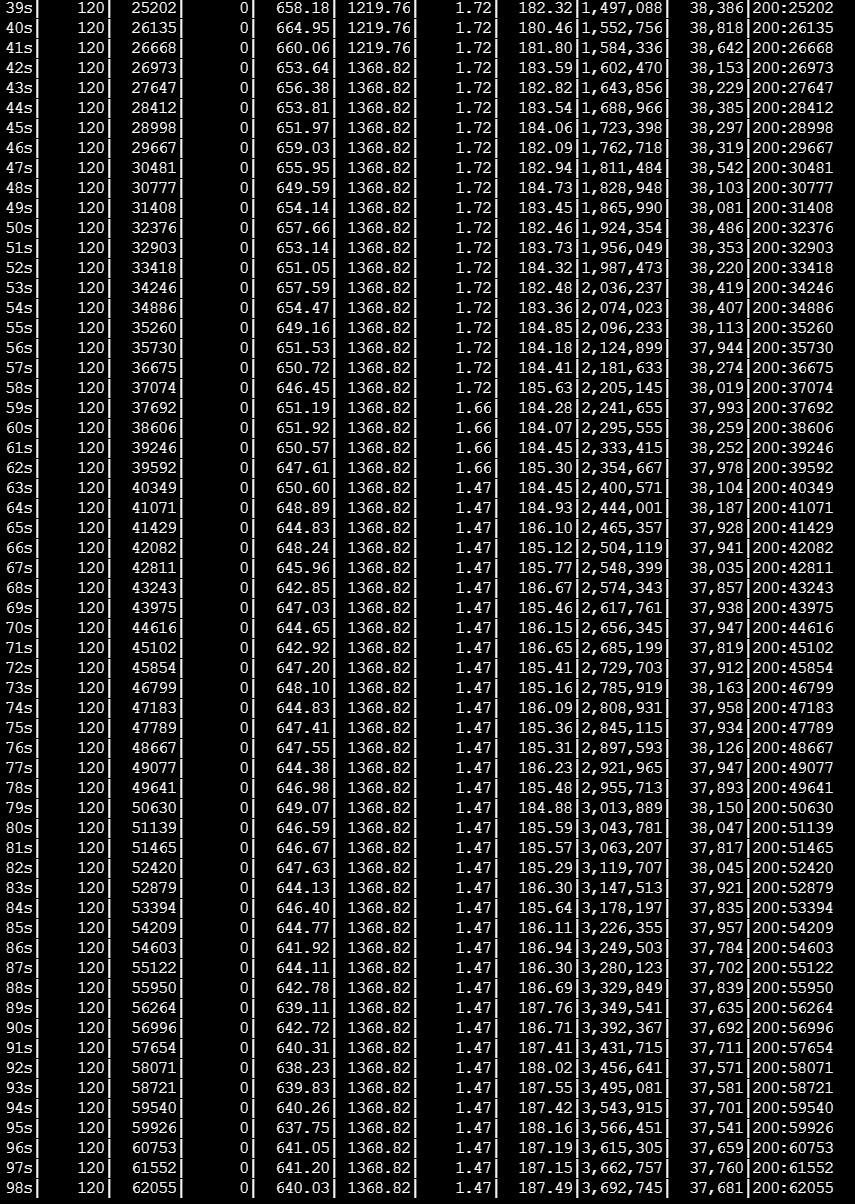
\includegraphics[width=0.9\textwidth]{6-3-1.jpg}
    \caption{压测过程}
    \label{压测过程}
\end{figure}
如上图6.8所示,显示了每一秒的接口压测过程,第6列是接口的QPS,可以发现是在640左右,响应时间均在1毫秒左右,返回状态码都是200。这一结果符合预期。

\begin{figure}[H]
    \centering
    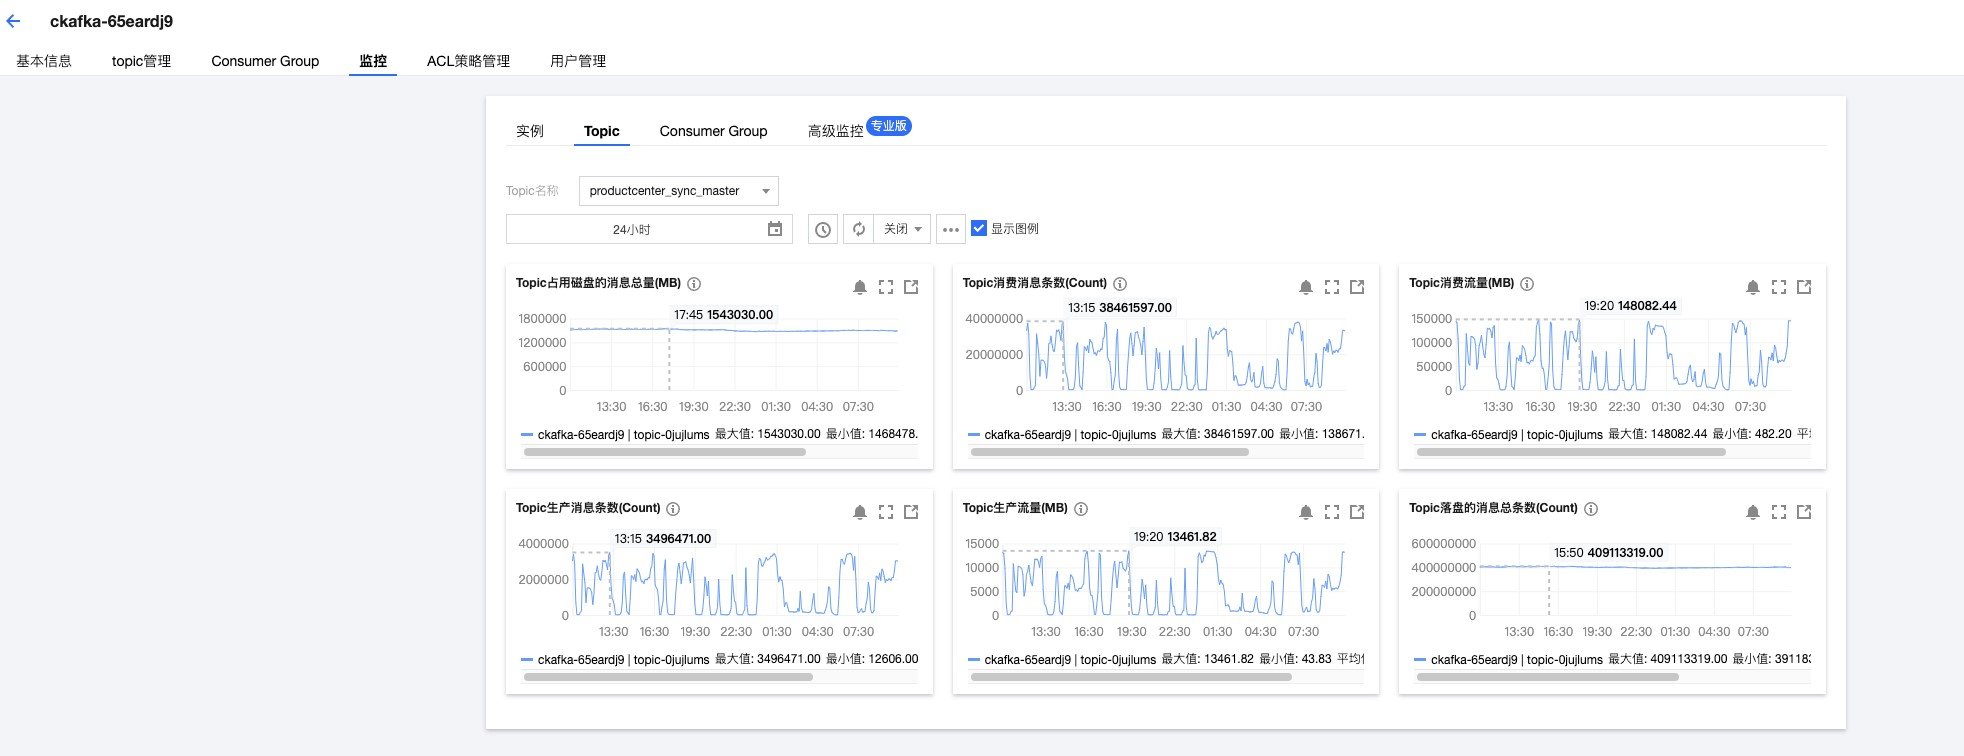
\includegraphics[width=0.9\textwidth]{6-3-2.jpg}
    \caption{监控状态}
    \label{监控状态}
\end{figure}
如上图6.9所示,显示了在压测过程中消息队列的消费情况,可以看出生产流量为13461MB左右,消费流量为148082MB左右,约为生产速度的11倍,表明当前有消息堆积,
但以目前的消息消费能力,可以消费完堆积的数据,这一结果符合预期。
%
%对StartExecution接口的Normal模式压测,并发数:120 请求数:20000000
%POST /v1/scheduler/StartExecution
%
%对StartExecution接口的Parallel模式压测,并发数:120 请求数:20000000
%POST /v1/scheduler/StartExecution


\section{本章小结}

本章阐述了对系统做了全方位的测试,包括功能性测试和功能性测试,确保了系统的设计功能的完备和可用,以及模拟大流量场景下系统表现的情况。
从结果上看,系统基本满足了需求分析要求的各项功能。 通过对系统整体的性能指标有了量化后的数据图表可供进一步分析,也为今后进一步
性能优化的方案设计提供重要的参考价值。